%! Author = gramic
%! Date = 22.04.24

% Preamble
\begin{flushleft}
    \subsection{YugabyteDB}
    \label{subsec:appendix_testing_yugabytedb}
    Zum einen, kann der Fehler irgendwann auftreten.\\
    In diesem Fall wird erst im Log die Fehlermeldung geworfen, dass die Zeitdifferenz zu gross ist:
    \begin{figure}[H]
        \centering
        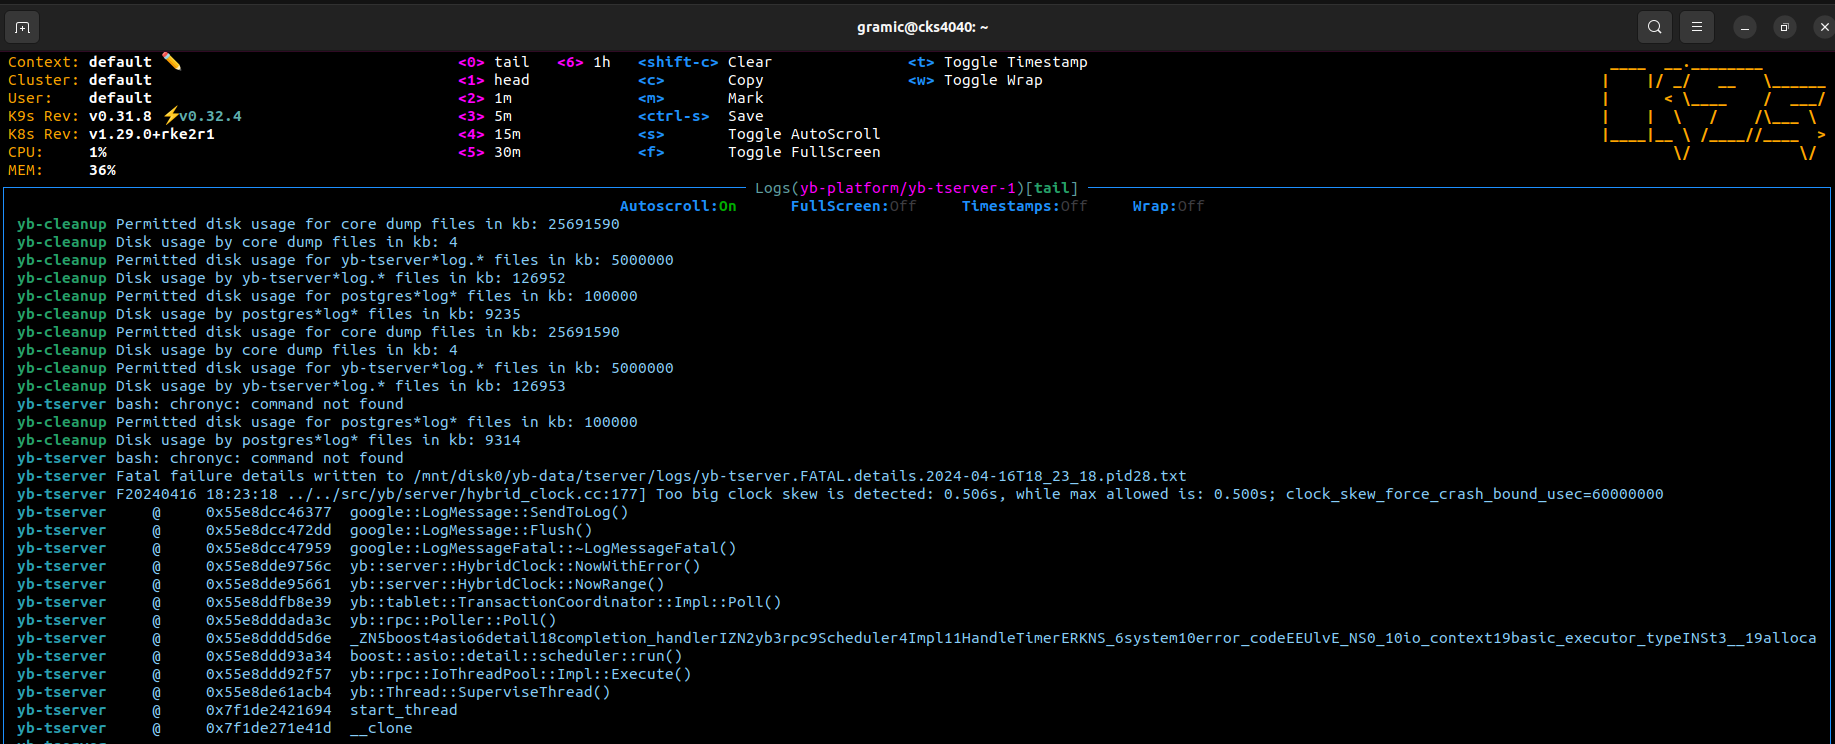
\includegraphics[width=1\linewidth]{source/appendix/evaluation_testing/yugabytedb_too_big_clock_skew_is_detected}
        \caption{YugabyteDB - Too big clock skew is detected}
        \label{fig:yugabytedb_too_big_clock_skew_is_detected}
    \end{figure}
    Eine folge ist, dass kein neuer Leader bestimmt werden kann:
    \begin{figure}[H]
        \centering
        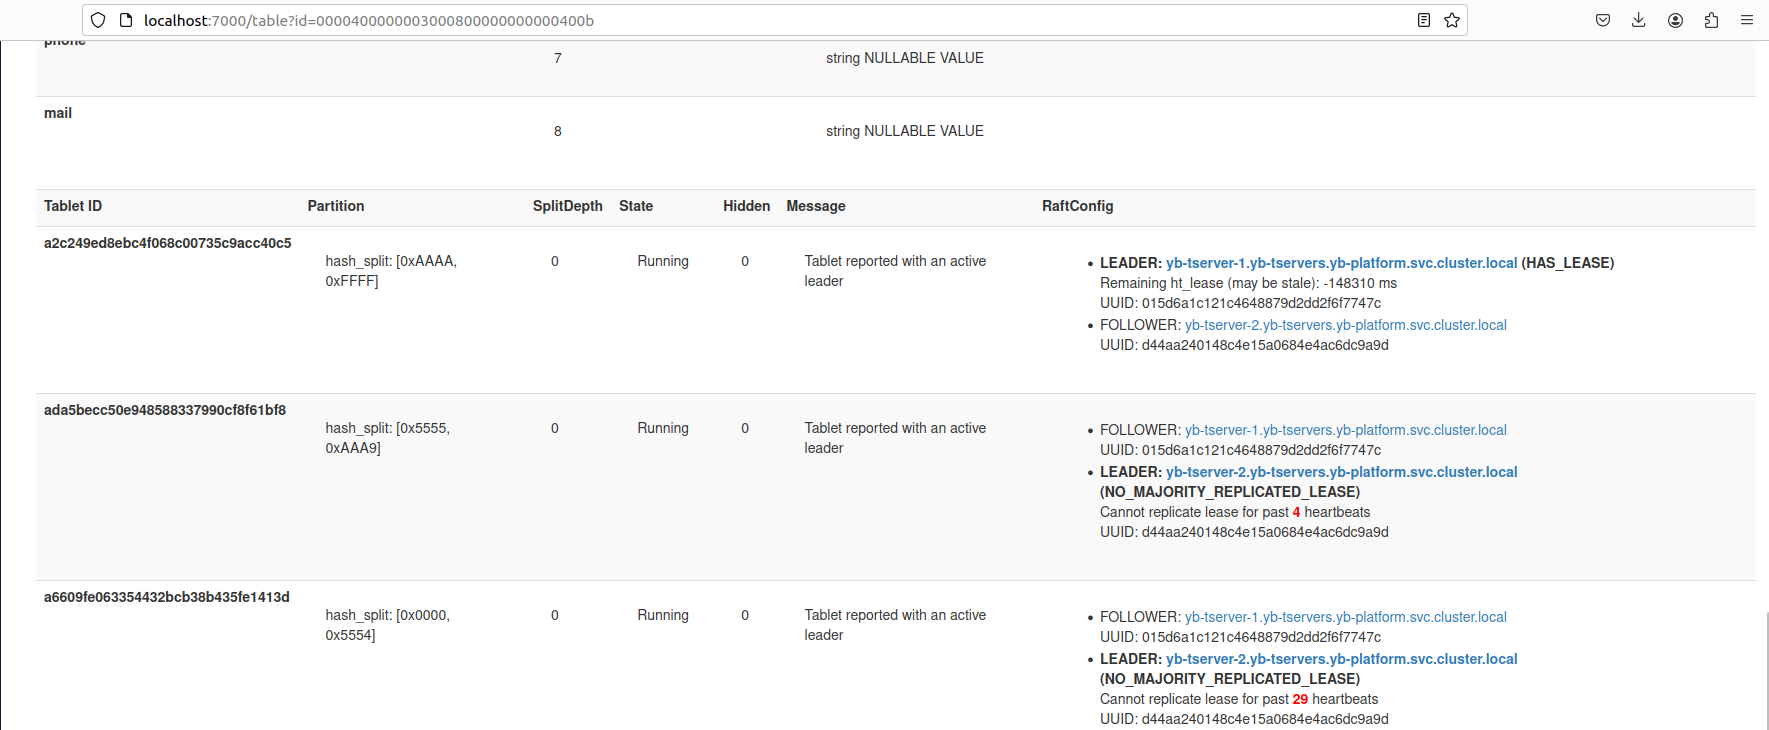
\includegraphics[width=1\linewidth]{source/appendix/evaluation_testing/yugabytedb_tablet_leader_lease}
        \caption{YugabyteDB - Tablet Leader - No Lease}
        \label{fig:yugabytedb_tablet_leader_lease}
    \end{figure}
    Als nächstes wird der komplette \texttt{tserver} in einem \texttt{CrashLoopBackOff} fallen:
    \begin{figure}[H]
        \centering
        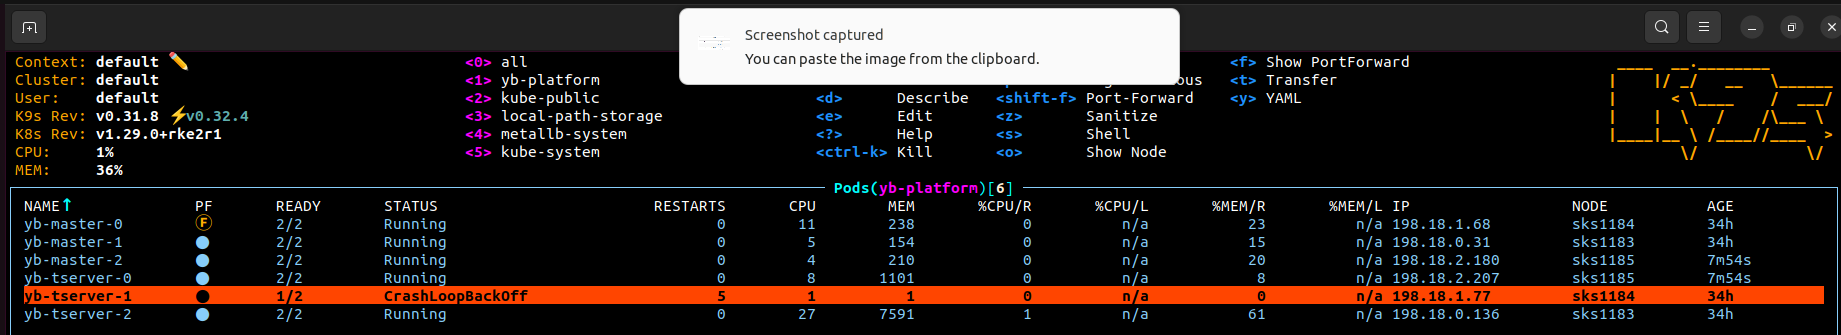
\includegraphics[width=1\linewidth]{source/appendix/evaluation_testing/yugabytedb_crashloopbackoff}
        \caption{YugabyteDB - CrashLoopBackOff}
        \label{fig:yugabytedb_crashloopbackoff}
    \end{figure}
    Der ganze Cluster an sich aber bleibt Arbeitsfähig.
\end{flushleft}
\begin{flushleft}
    Anders sieht es aus, wenn auch \texttt{tmaster}-Nodes von Start weg betroffen sind.\\
    Es werden aber primär nur die Logs überall geschrieben:
    \begin{figure}[H]
        \centering
        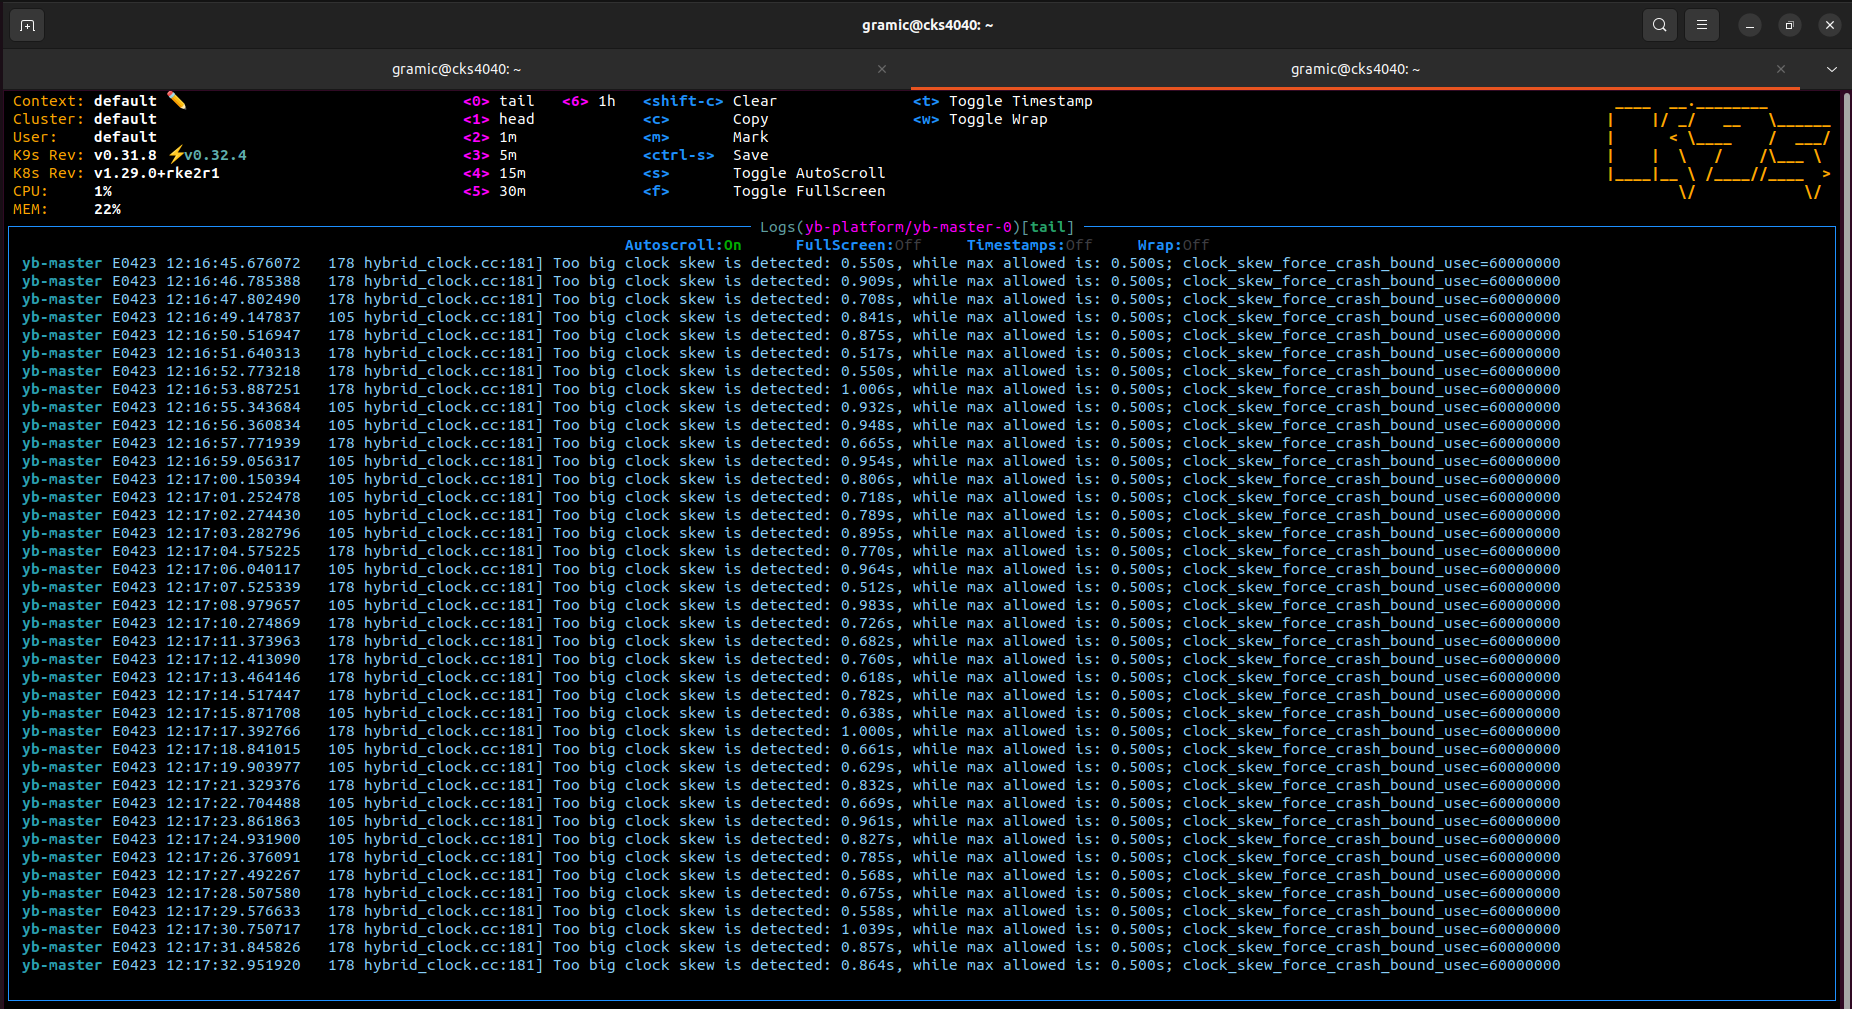
\includegraphics[width=1\linewidth]{source/appendix/evaluation_testing/yugabytedb_yb-tmaster-0_sks1184_clock_error}
        \caption{YugabyteDB - Too big clock skew is detected - tmaster}
        \label{fig:yugabytedb_yb-tmaster-0_sks1184_clock_error}
    \end{figure}
    \begin{figure}[H]
        \centering
        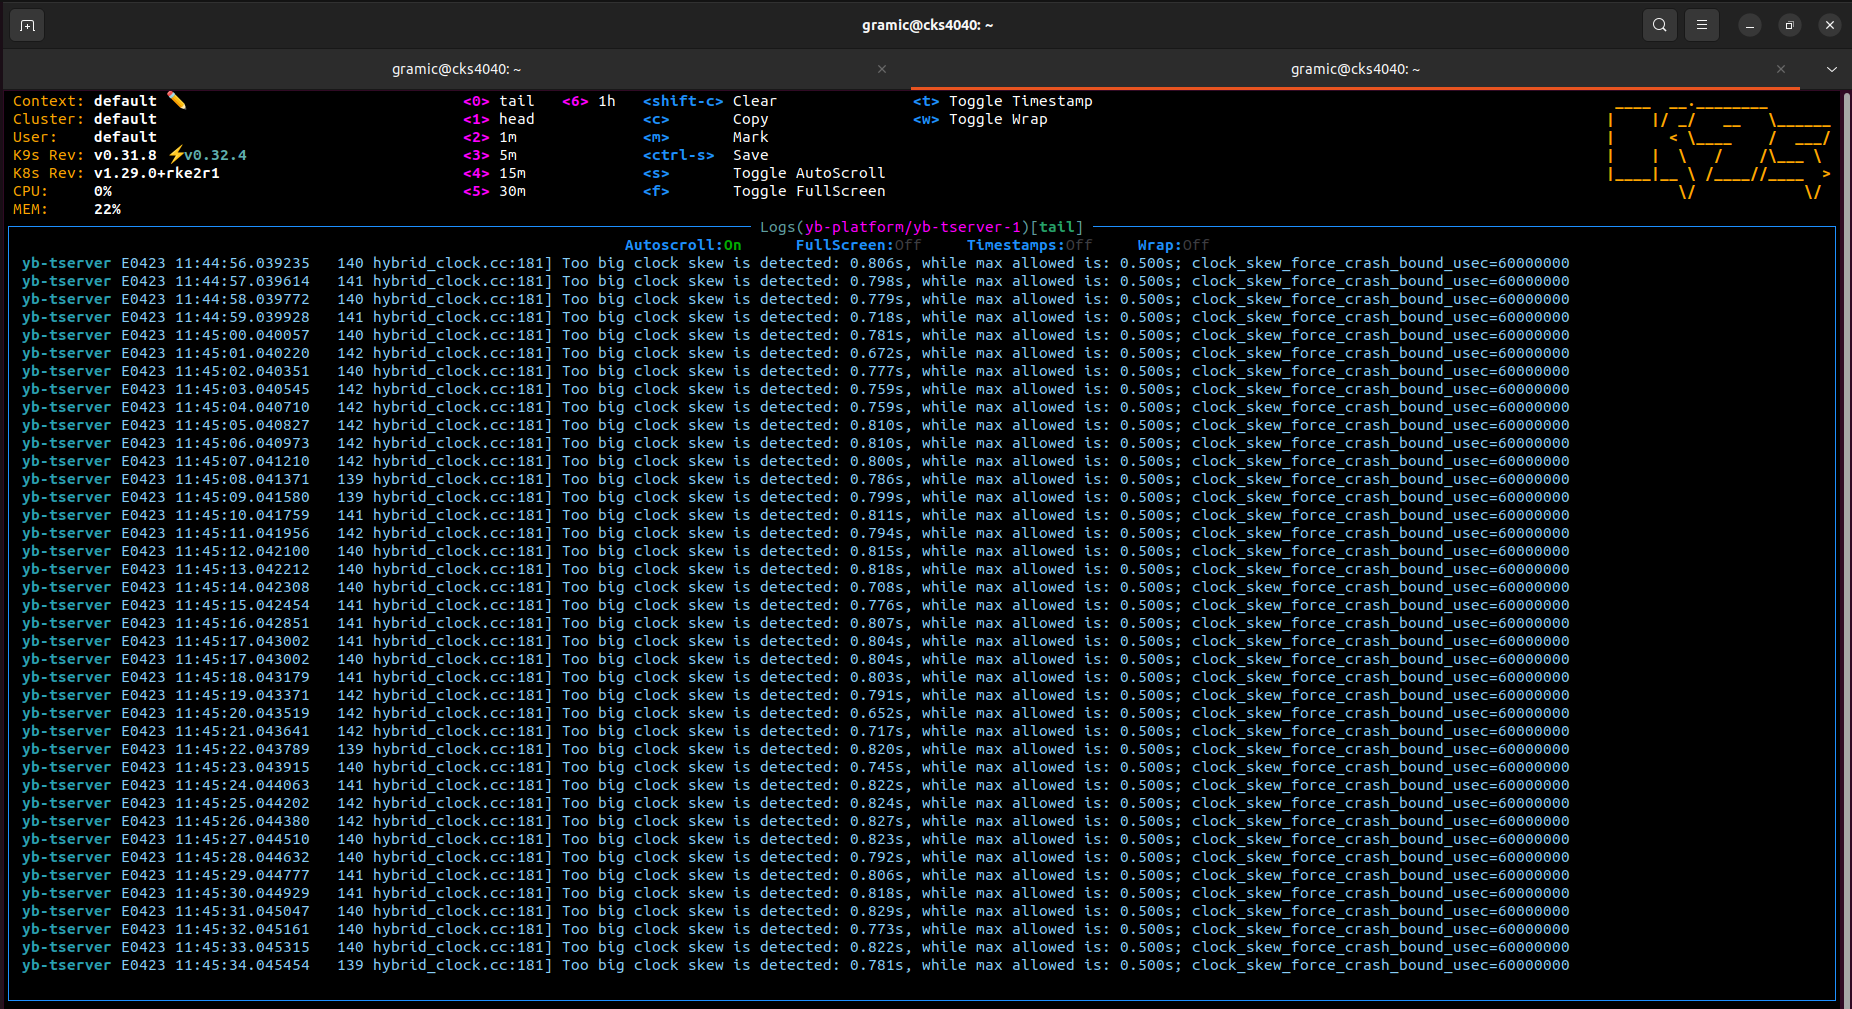
\includegraphics[width=1\linewidth]{source/appendix/evaluation_testing/yugabytedb_yb-tserver-1_sks1184_clock_error}
        \caption{YugabyteDB - Too big clock skew is detected - tserver}
        \label{fig:yugabytedb_yb-tserver-1_sks1184_clock_error}
    \end{figure}
%    \begin{figure}[H]
%        \centering
%        \subfloat[yb-tmaster-0]{{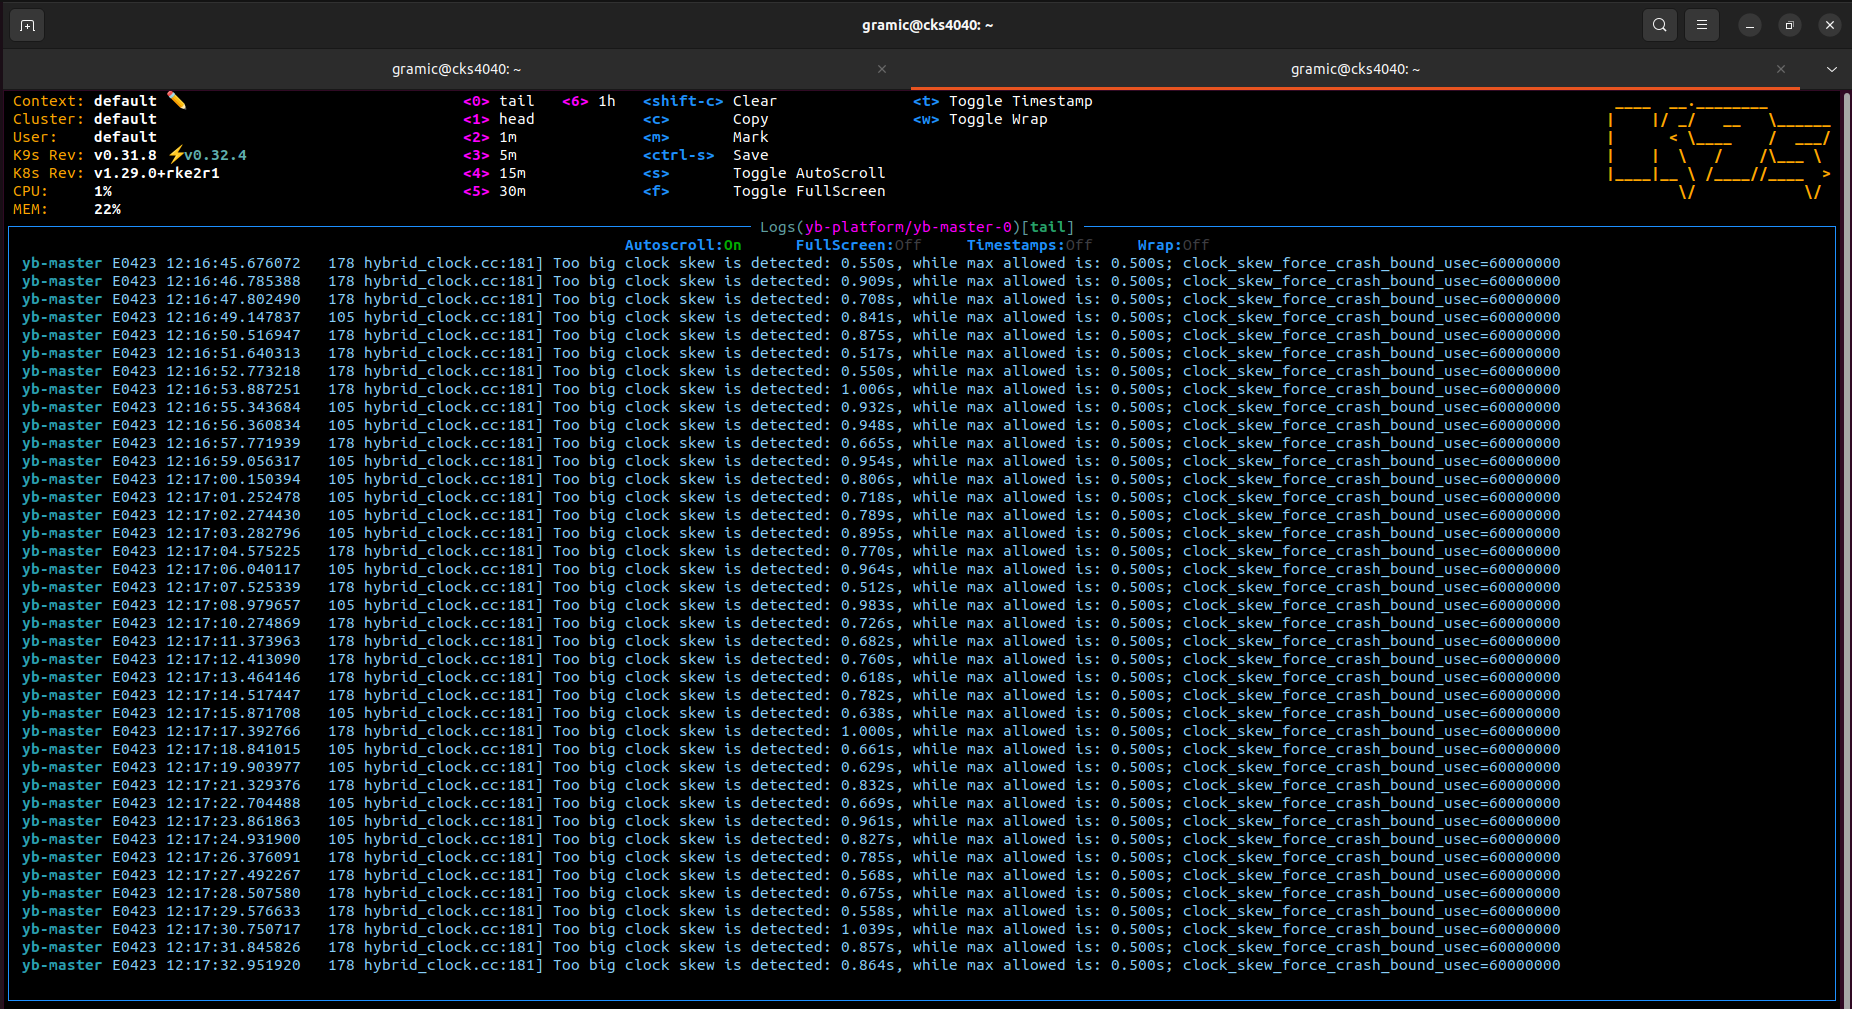
\includegraphics[width=0.47\linewidth]{source/appendix/evaluation_testing/yugabytedb_yb-tmaster-0_sks1184_clock_error} }}%
%        \qquad
%        \subfloat[yb-tserver-1]{{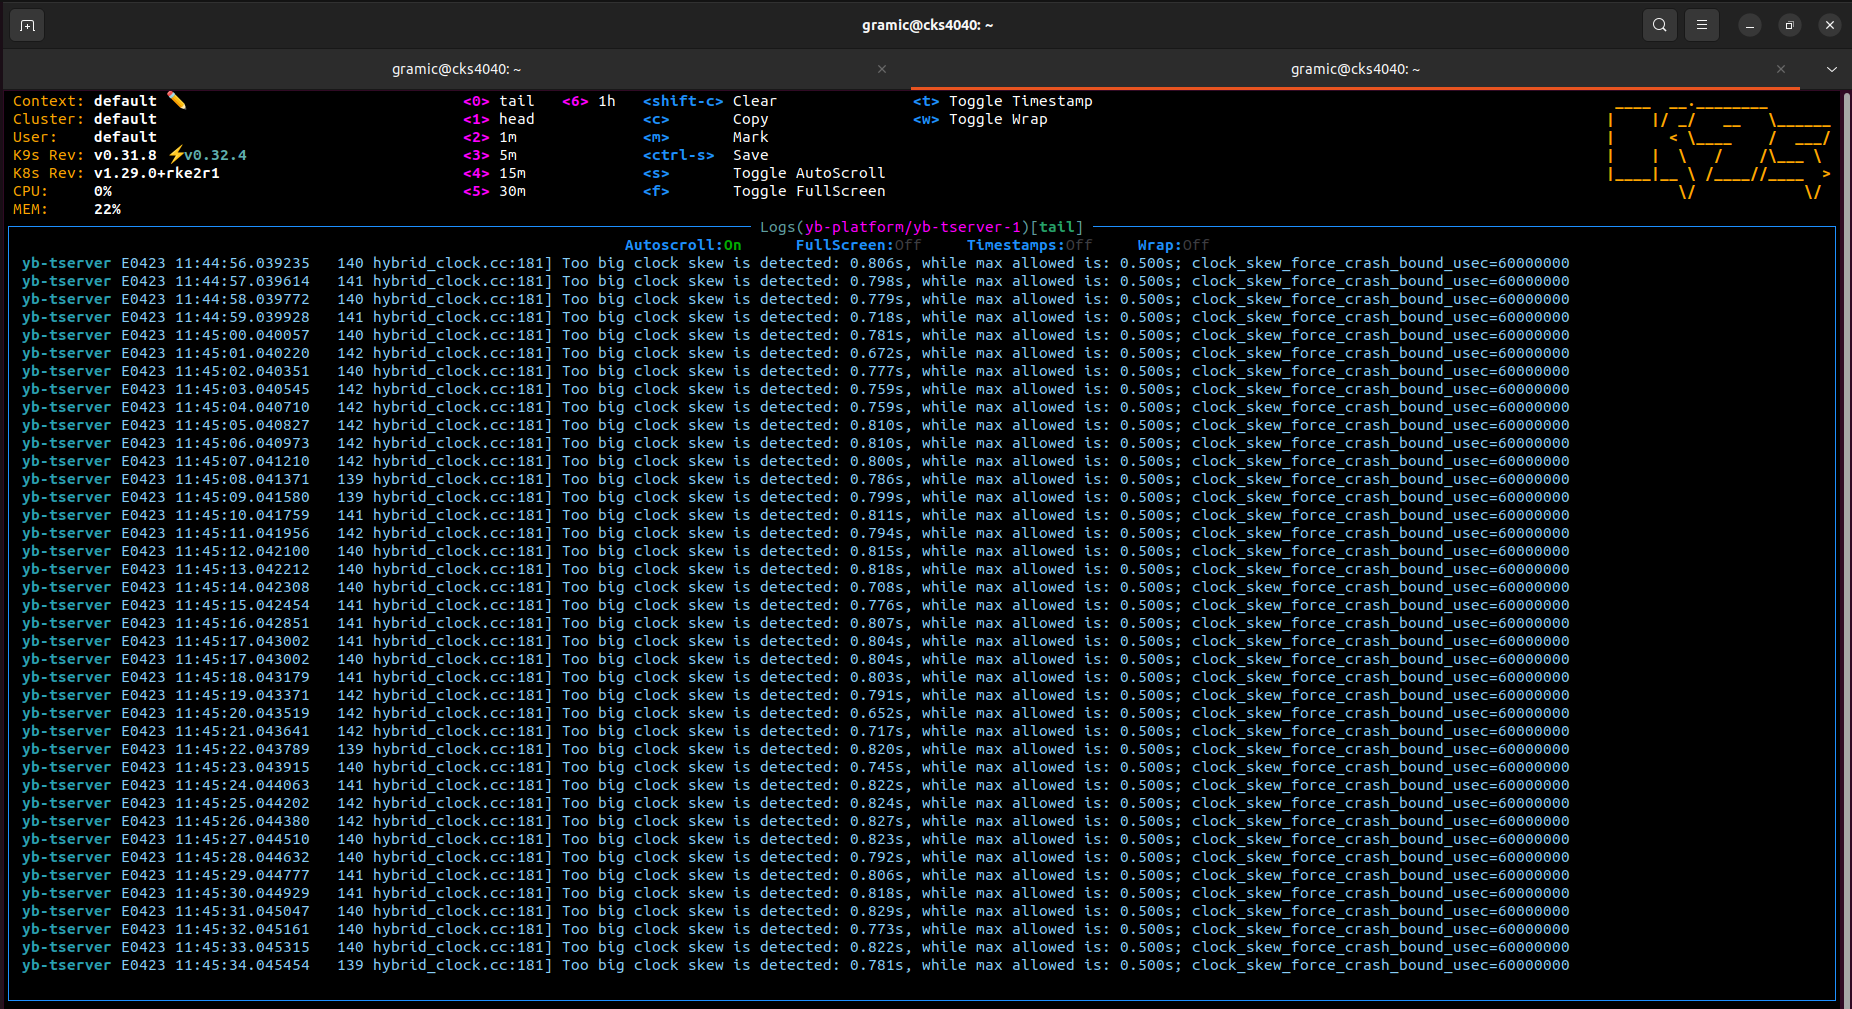
\includegraphics[width=0.47\linewidth]{source/appendix/evaluation_testing/yugabytedb_yb-tserver-1_sks1184_clock_error} }}%
%        \caption{YugabyteDB - Too big clock skew is detected - Node}
%        \label{fig:yugabytedb_sks1184_clock_error}
%    \end{figure}
    YugabyteDB erlaubt in so einem Fall keine Zugriffe mehr auf den Cluster.\\
    So wird verhindert, dass der Cluster korrumpiert wird.
\end{flushleft}